\documentclass{article}

\usepackage{titlesec}
\usepackage{longtable}
\usepackage{array} % for defining a new column type
\usepackage{varwidth} %for the varwidth minipage environment
\usepackage{color, colortbl}
\usepackage{caption}
\usepackage{subfigure}
\usepackage{filecontents}
\usepackage[section]{placeins}
\usepackage{float}
\usepackage{lscape}

\definecolor{Gray}{gray}{0.9}

\usepackage{pgf-umlsd}
\usepackage{pgf-umlcd}
\newcommand{\sectionbreak}{\clearpage}

\begin{document}

\newcolumntype{M}{>{\begin{varwidth}{4cm}}l<{\end{varwidth}}} %M is for Maximal column

\begin{titlepage}
	\Huge{Bitcode Assignment 2}
\end{titlepage}


\section{Design Patterns}
Using design patterns in software project is a good practice. It helps to make your software understandable, sustainable and expendable. We have chosen two design patterns and implemented them in our existing code, the observer pattern and the factory pattern.

\subsection{The Observer Design Pattern}
tbd {explain why}

\subsubsection{Factory Class Diagrams}
tbd
\begin{figure}[H]
	\centering
	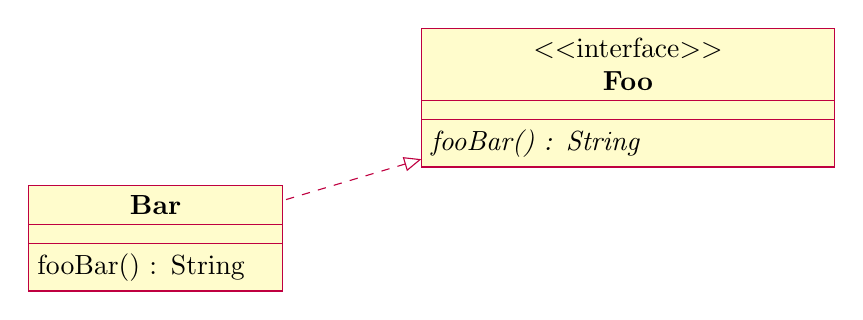
\begin{tikzpicture}
	\begin{interface}{Foo}{0,0}
	\operation[0]{fooBar() : String}
	\end{interface}
	\begin{class}[text width = 3cm]{Bar}{-6,-2}
	\implement{Foo}
	\operation{fooBar() : String}
	\end{class}
	\end{tikzpicture}
\end{figure}

\subsubsection{Observer Sequence Diagram}
tbd
\begin{figure}[H]
	\centering
	\begin{sequencediagram}
		\newthread{A}{foo}{}
		\newthread{B}{bar}{}
		\begin{call}{A}{FooBar}{B}{}
		\end{call}{B}{BarFoo}{A}
	\end{sequencediagram}
\end{figure}

\subsection{The Factory Design Pattern}
tbd {explain why} 

\subsubsection{Factory Class Diagrams}
tbd
\begin{figure}[H]
	\centering
	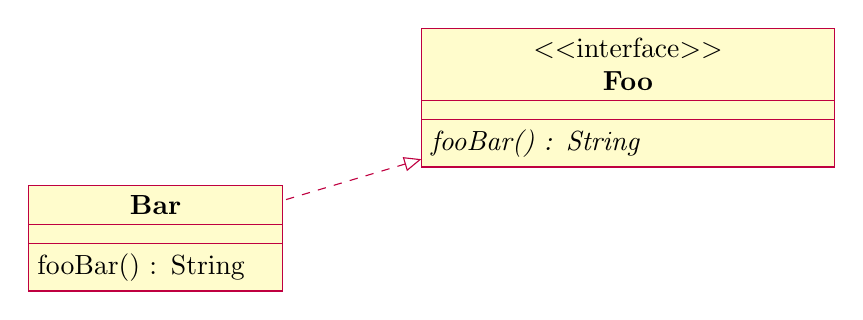
\begin{tikzpicture}
	\begin{interface}{Foo}{0,0}
	\operation[0]{fooBar() : String}
	\end{interface}
	\begin{class}[text width = 3cm]{Bar}{-6,-2}
	\implement{Foo}
	\operation{fooBar() : String}
	\end{class}
	\end{tikzpicture}
\end{figure}

\subsubsection{Factory Sequence Diagram}
tbd
\begin{figure}[H]
	\centering
	\begin{sequencediagram}
		\newthread{A}{foo}{}
		\newthread{B}{bar}{}
		\begin{call}{A}{FooBar}{B}{}
		\end{call}{B}{BarFoo}{A}
	\end{sequencediagram}
\end{figure}

\section{Your wish is my command}
Our client wanted to have two new features implemented, which consist of a high score page and maximum amount of moves per level. For each each feature we have created new requirements and a software design.

\subsection{High Score Page}
tbd

\subsubsection{Requirements}
tbd

\subsubsection{Software Design}
tbd {use UML}

\subsection{Maximum Moves per Level}
tbd

\subsubsection{Requirements}
tbd

\subsubsection{Software Design}
tbd {use UML}


\section{Turn-based Multiplayer}
In exercise three we have been asked to implement a feature that we wanted to implement. We have chosen to implement turn-based Multiplayer. For this feature we also created new requirements and a software design.

\subsection{Requirements}
tbd

\subsection{Software Design}
tbd {use UML}



\end{document}






